\chapter{Konzeption}

Um eine Basis zur Umsetzung des \textit{Smart Warehouse} Szenarios zu schaffen, sind zunächst einige konzeptionelle Überlegungen notwendig, die in diesem Kapitel betrachtet werden sollen. Sie beschränken sich im Wesentlichen auf sechs übergeordnete Themenbereiche, die in Abbildung \ref{schritte} dargestellt sind. 

\begin{figure}[ht]
	\begin{center}
		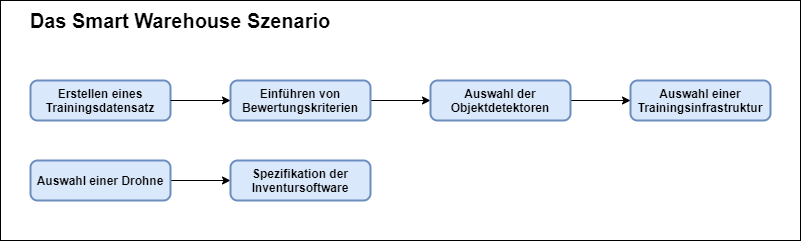
\includegraphics[width=15cm]{Bilder/blockdiagramm.png} 
		\caption[Konzeptionelle Schritte]{Konzeptionelle Schritte}
		\label{schritte}
	\end{center}
\end{figure}

Daraus ergeben sich zwei Neuheitswerte. Zum einen soll evaluiert werden, ob die bestehenden Objektdetektoren für industrielle Anwendungsszenarien grundsätzlich geeignet sind, zum anderen, ob das spezifische Anwendungsszenario zur automatisierten Durchführung einer Inventur von Warenhäusern mit einer Drohne prototypisch umsetzbar ist.

Für das \textit{Smart Warehouse} Szenario ist demnach zum einen die Entwicklung eines \textit{Deep Learning} Modells notwendig, das auf das Anwendungsszenario einer Inventur von Warenhäusern spezialisiert ist. Hierzu muss ein geeigneter Trainingsdatensatz erstellt werden, auf dem die ausgewählten Objektdetektoren trainiert werden sollen. Um die Objektdetektoren miteinander vergleichen zu können, ist zudem die Einführung von Bewertungskriterien notwendig. Auf Basis dieser Kriterien wird später evaluiert, ob die ausgewählten Objektdetektoren sich allgemein für einen industriellen Einsatz eignen. Welche Objektdetektoren überhaupt im Sinne des \textit{Smart Warehouse} Szenarios miteinander verglichen werden sollen, ist im nächsten Schritt \glqq Auswahl der Objektdetektoren\grqq{} zu beschließen. Anschließend stellt sich nur noch die Frage, auf welcher Infrastruktur die Objektdetektoren trainiert werden sollen.

Um das zweite Ziel der Arbeit zu erarbeiten, kann auf den Ergebnissen des ersten Ziels aufgebaut werden. Eine Drohne soll die benötigten Daten zur Inferenz liefern. Welche Drohne dies sein soll, ist im ersten Schritt zu erarbeiten. Die Drohne soll über eine Webapplikation ansprechbar sein, auf der zudem die Ergebnisse der Inventur präsentiert werden sollen. Diese Inventursoftware ist im letzten Schritt in ihrem Umfang zu spezifizieren.

\section{Erstellen eines Trainingsdatensatzes}

Das \textit{Smart Warehouse} lehnt sich an ein großes Warenhaus an, bei dem Produkte nicht in Kartons verpackt, sondern als ganzes auf Regalen angeordnet sind, ähnlich wie bei Warenhäusern wie \textit{Baumarkt} oder \textit{Selgros}. Bei dem Aufbau des Trainingsdatensatzes hat die Machbarkeitsstudie allerdings nicht zum Ziel, ein solches Warenhaus vollständig im Datensatz abzubilden, sondern wesentlich den Datensatz so umfangreich zu wählen, um eine generelle Umsetzbarkeit des \textit{Smart Warehouse} Szenarios zu beweisen. Im Rahmen des Projektes wurde sich deshalb exemplarisch auf Getränkeflaschen eines Warenhauses konzentriert. Dabei wurden neun Kategorien festgelegt (siehe Abbildung \ref{categories}). 

\begin{figure}[ht]
	\subfigure[Saskia Wasser Klein]{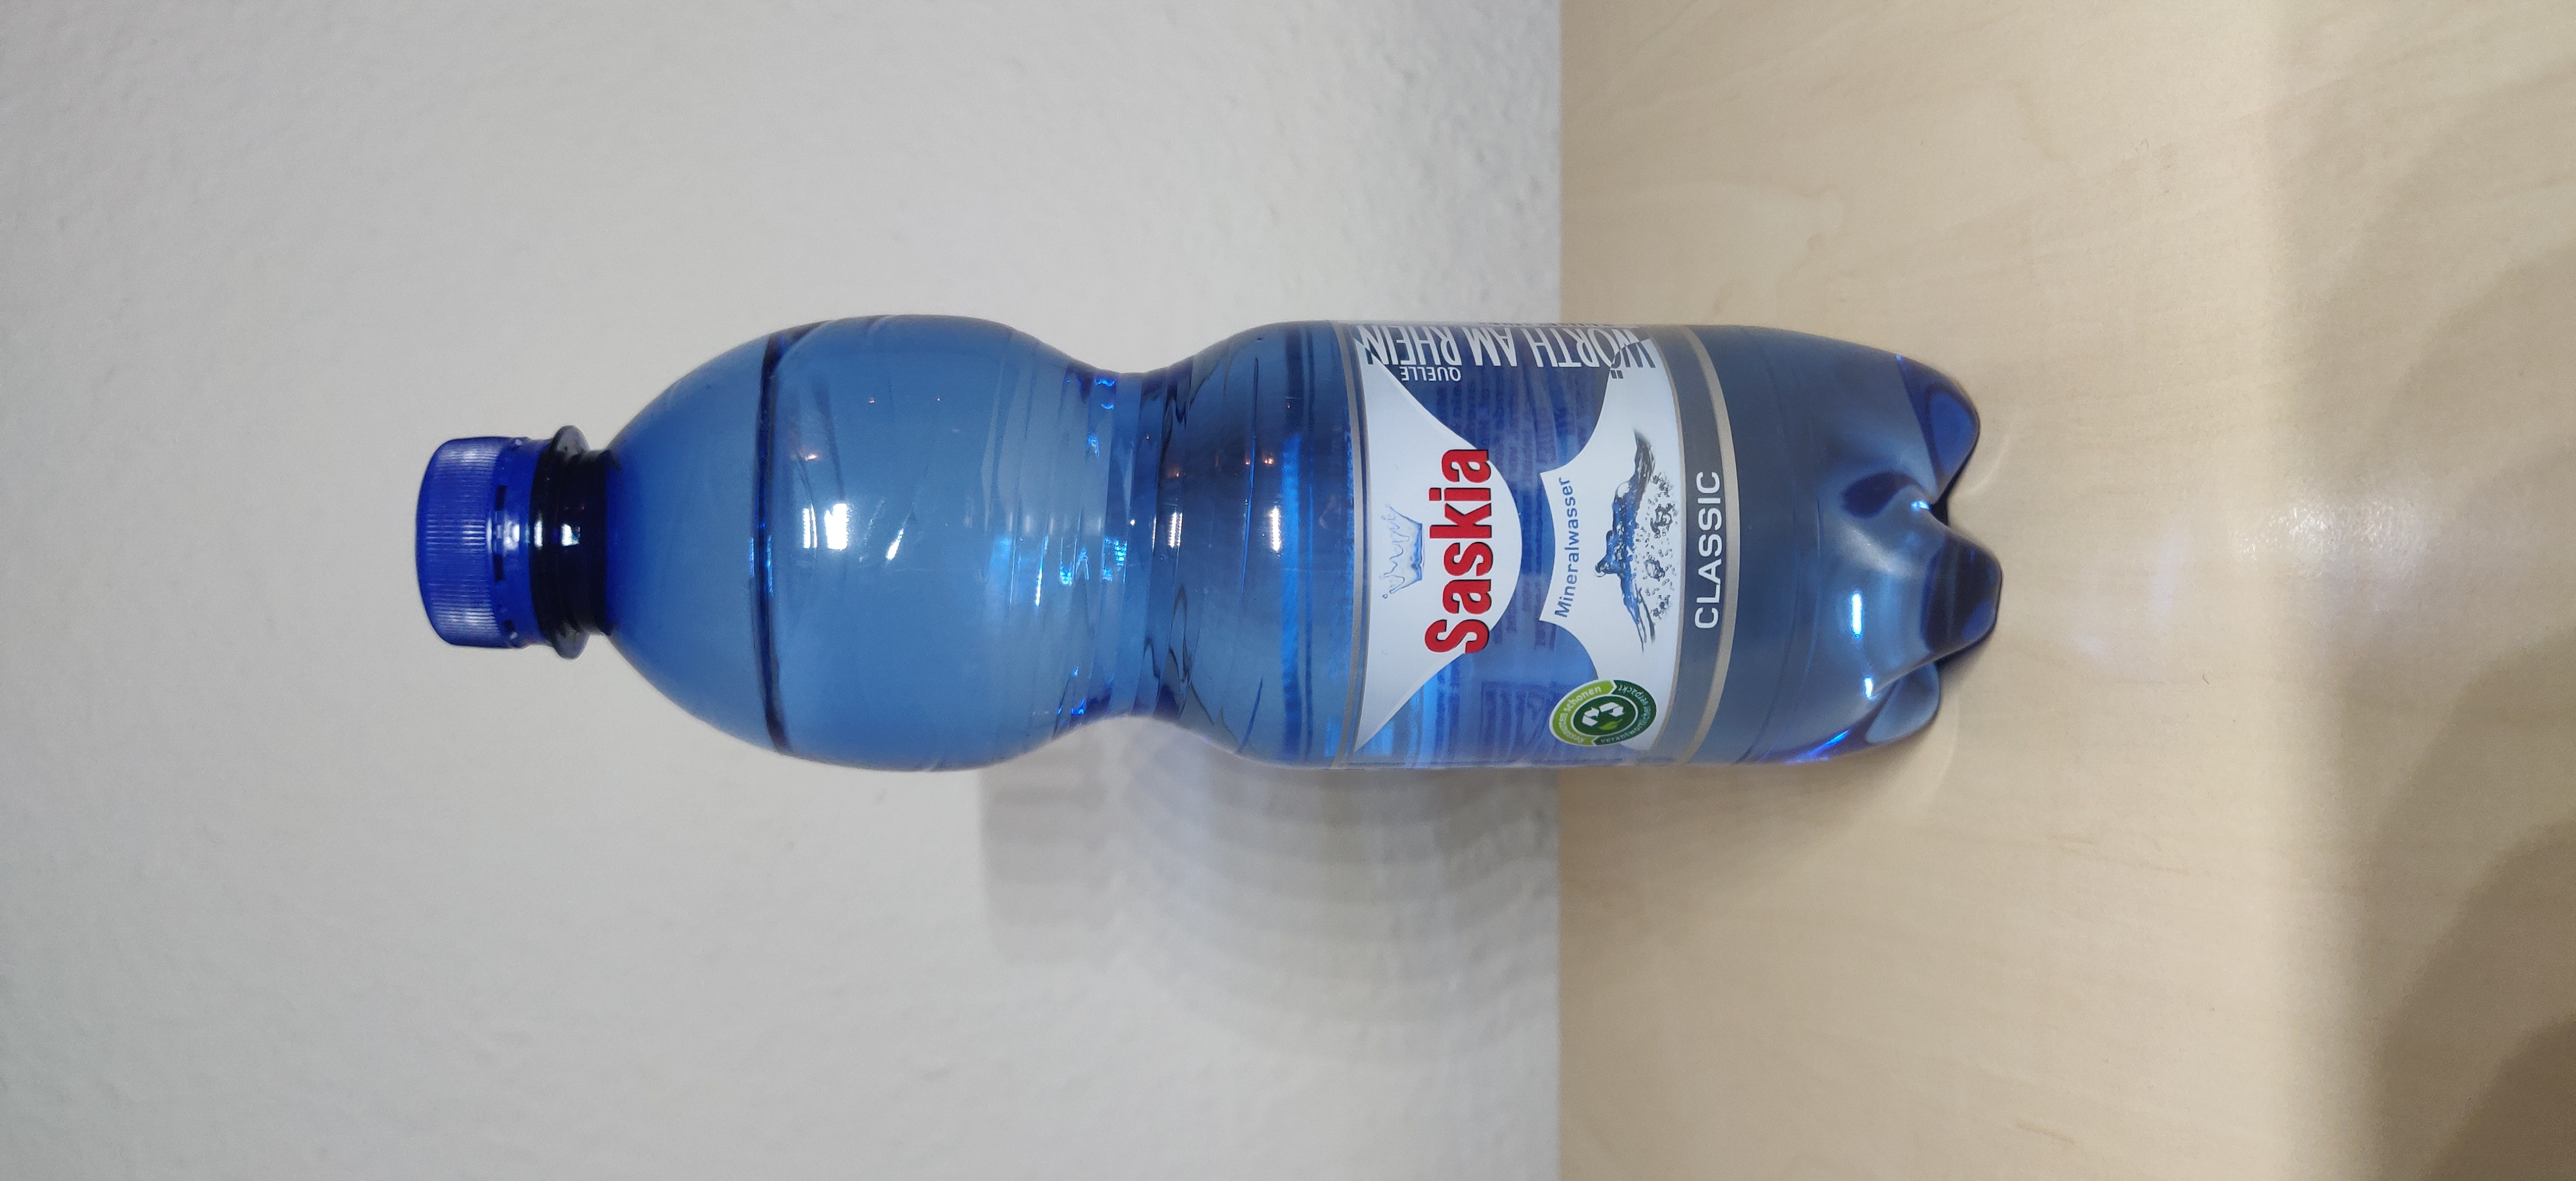
\includegraphics[width=0.30\textwidth]{Bilder/wasser_klein.jpg}}\hfill
	\subfigure[Saskia Wasser Groß]{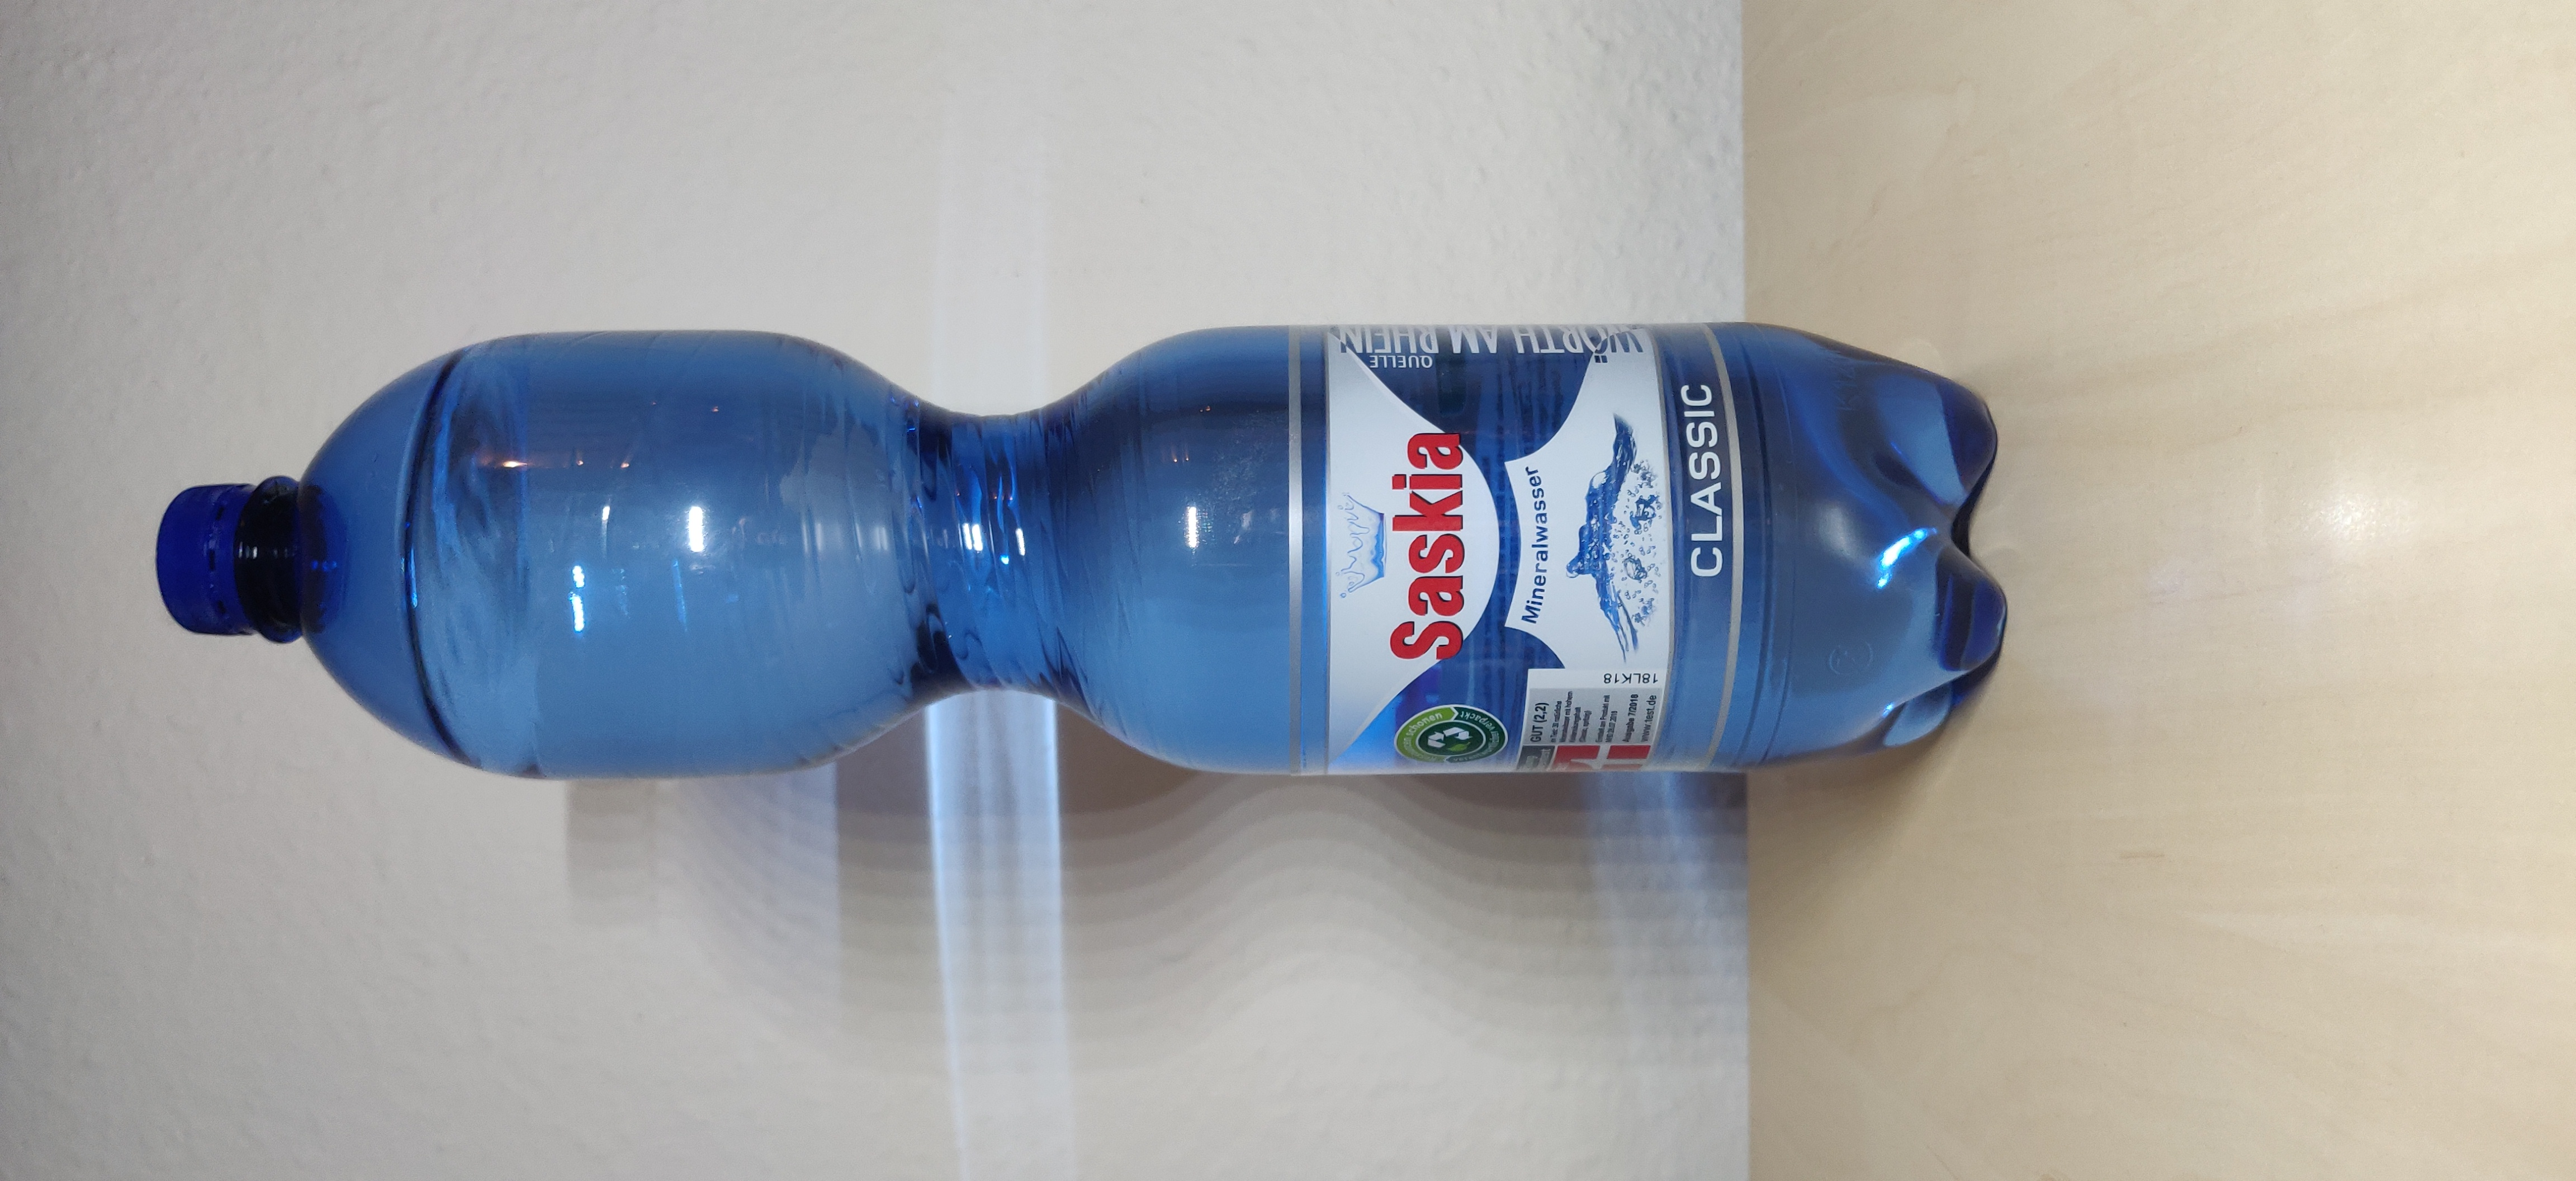
\includegraphics[width=0.30\textwidth]{Bilder/wasser_gross.jpg}}\hfill
	\subfigure[Pepsi Cola Klein]{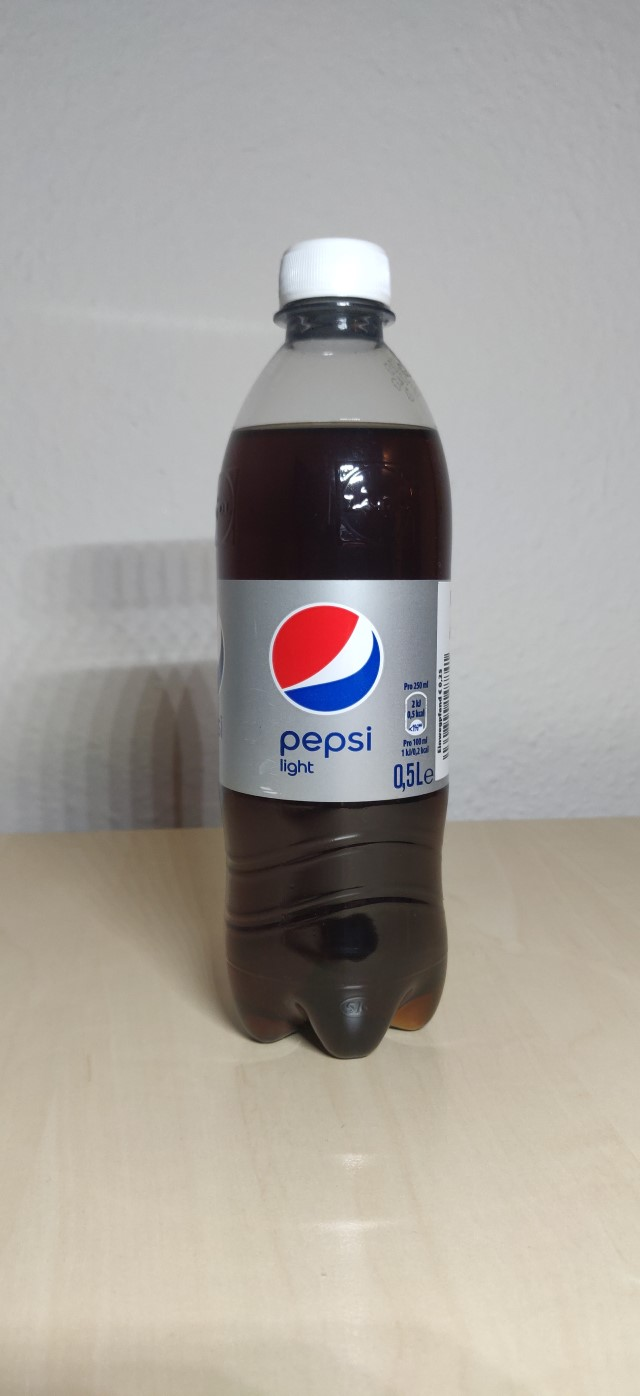
\includegraphics[width=0.30\textwidth]{Bilder/cola_klein.jpg}}\hfill
	\subfigure[Pepsi Cola Groß]{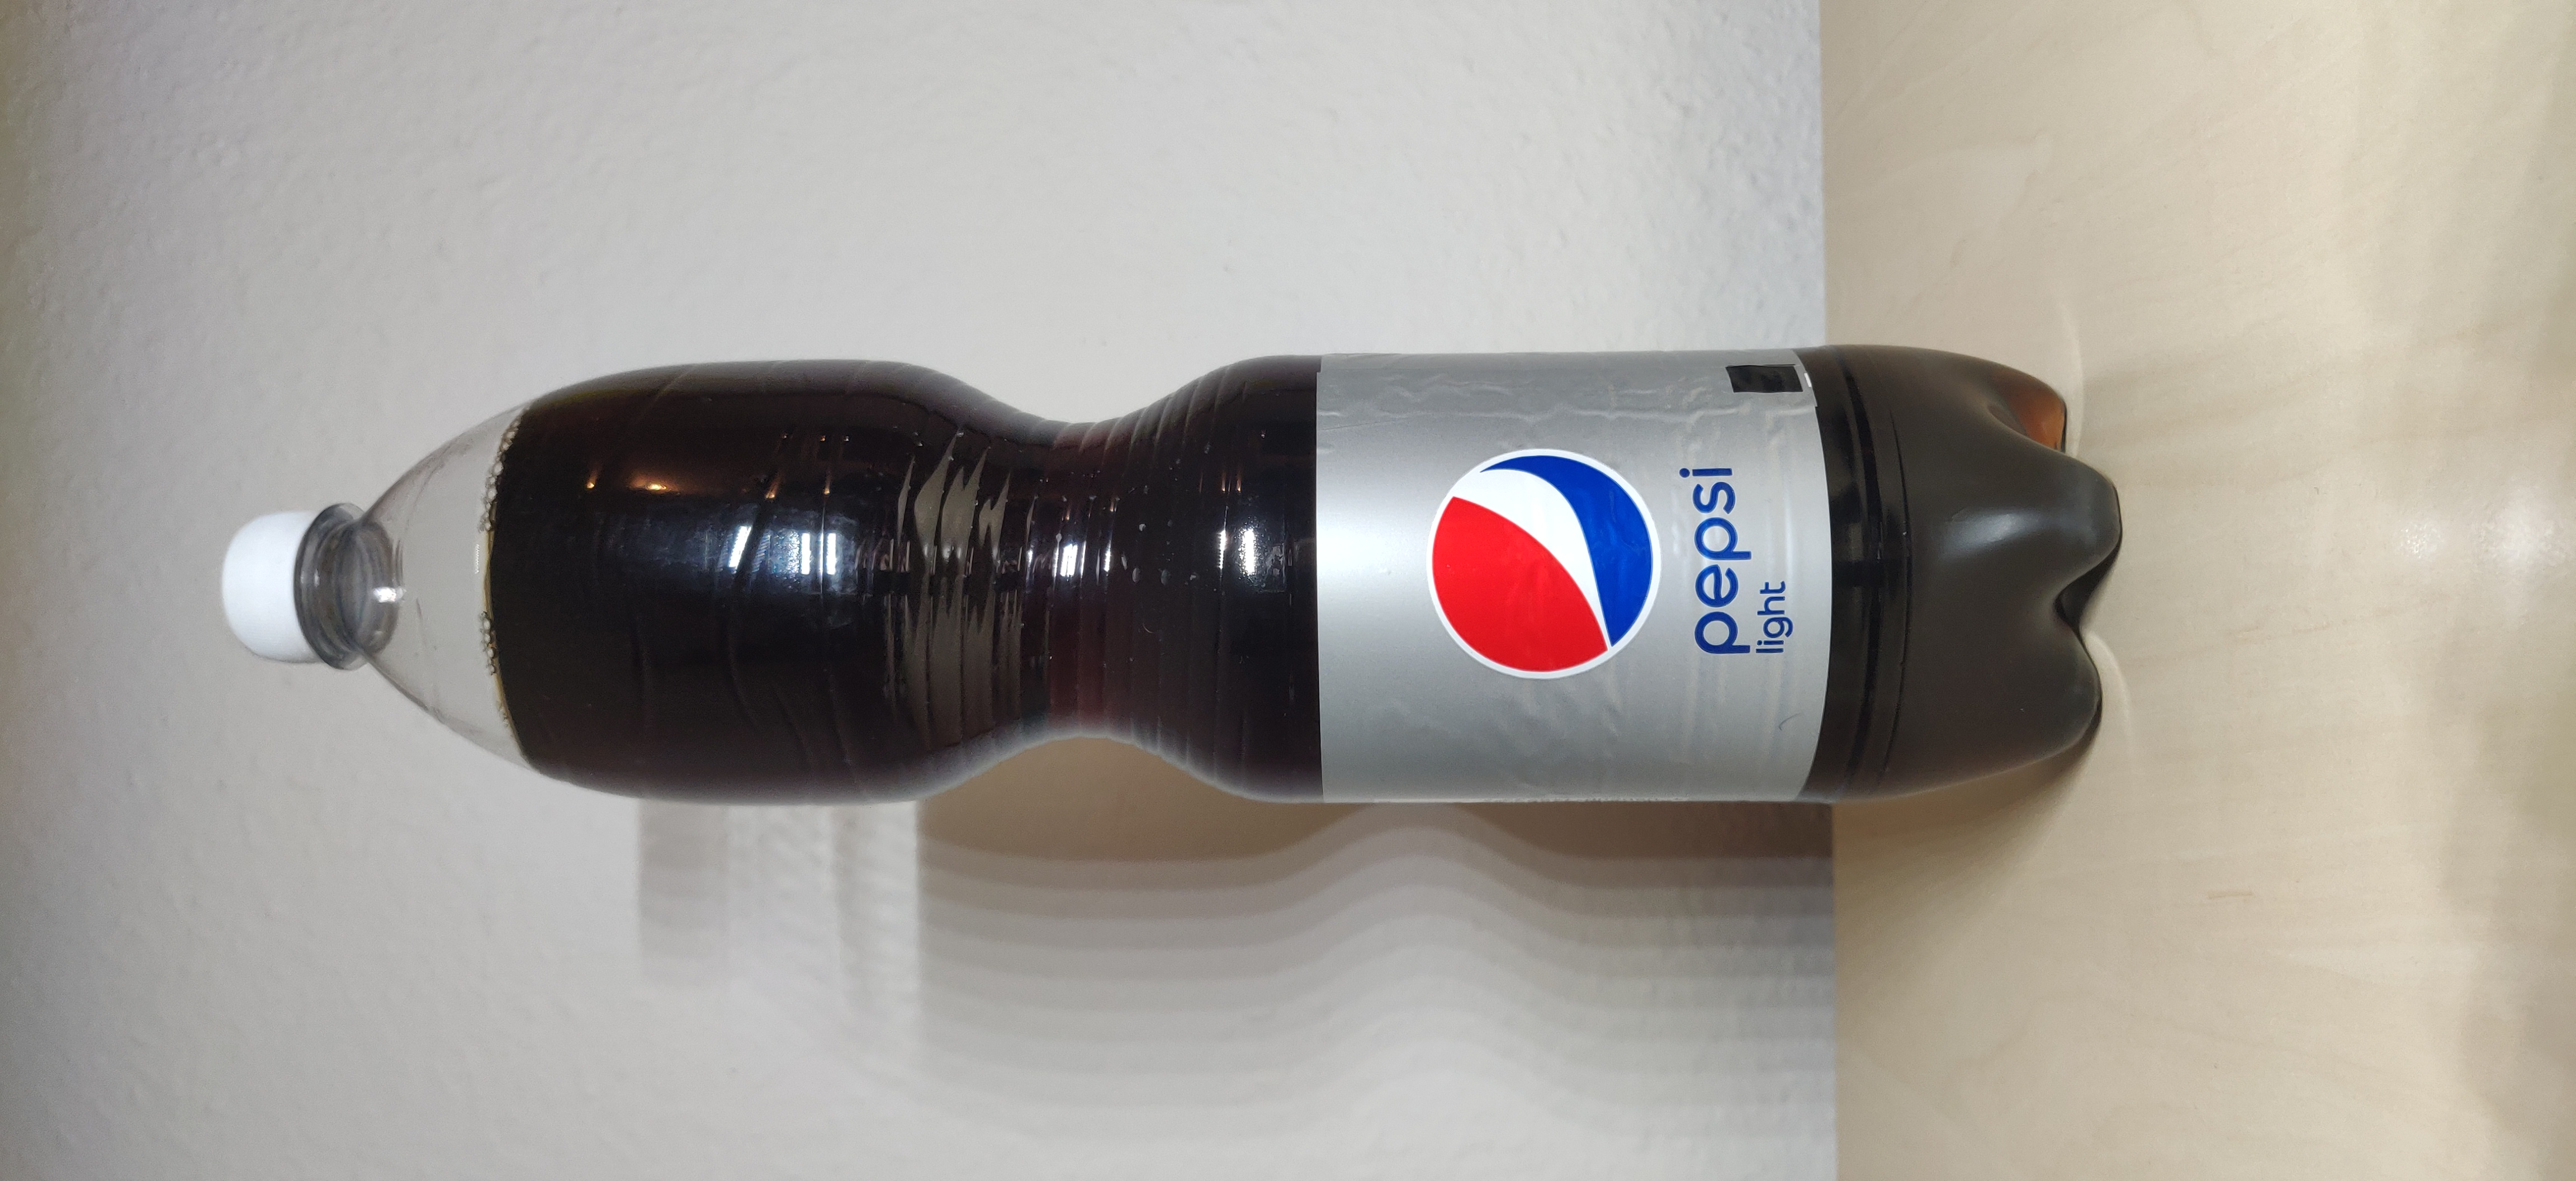
\includegraphics[width=0.30\textwidth]{Bilder/cola_gross.jpg}}\hfill
	\subfigure[ISO]{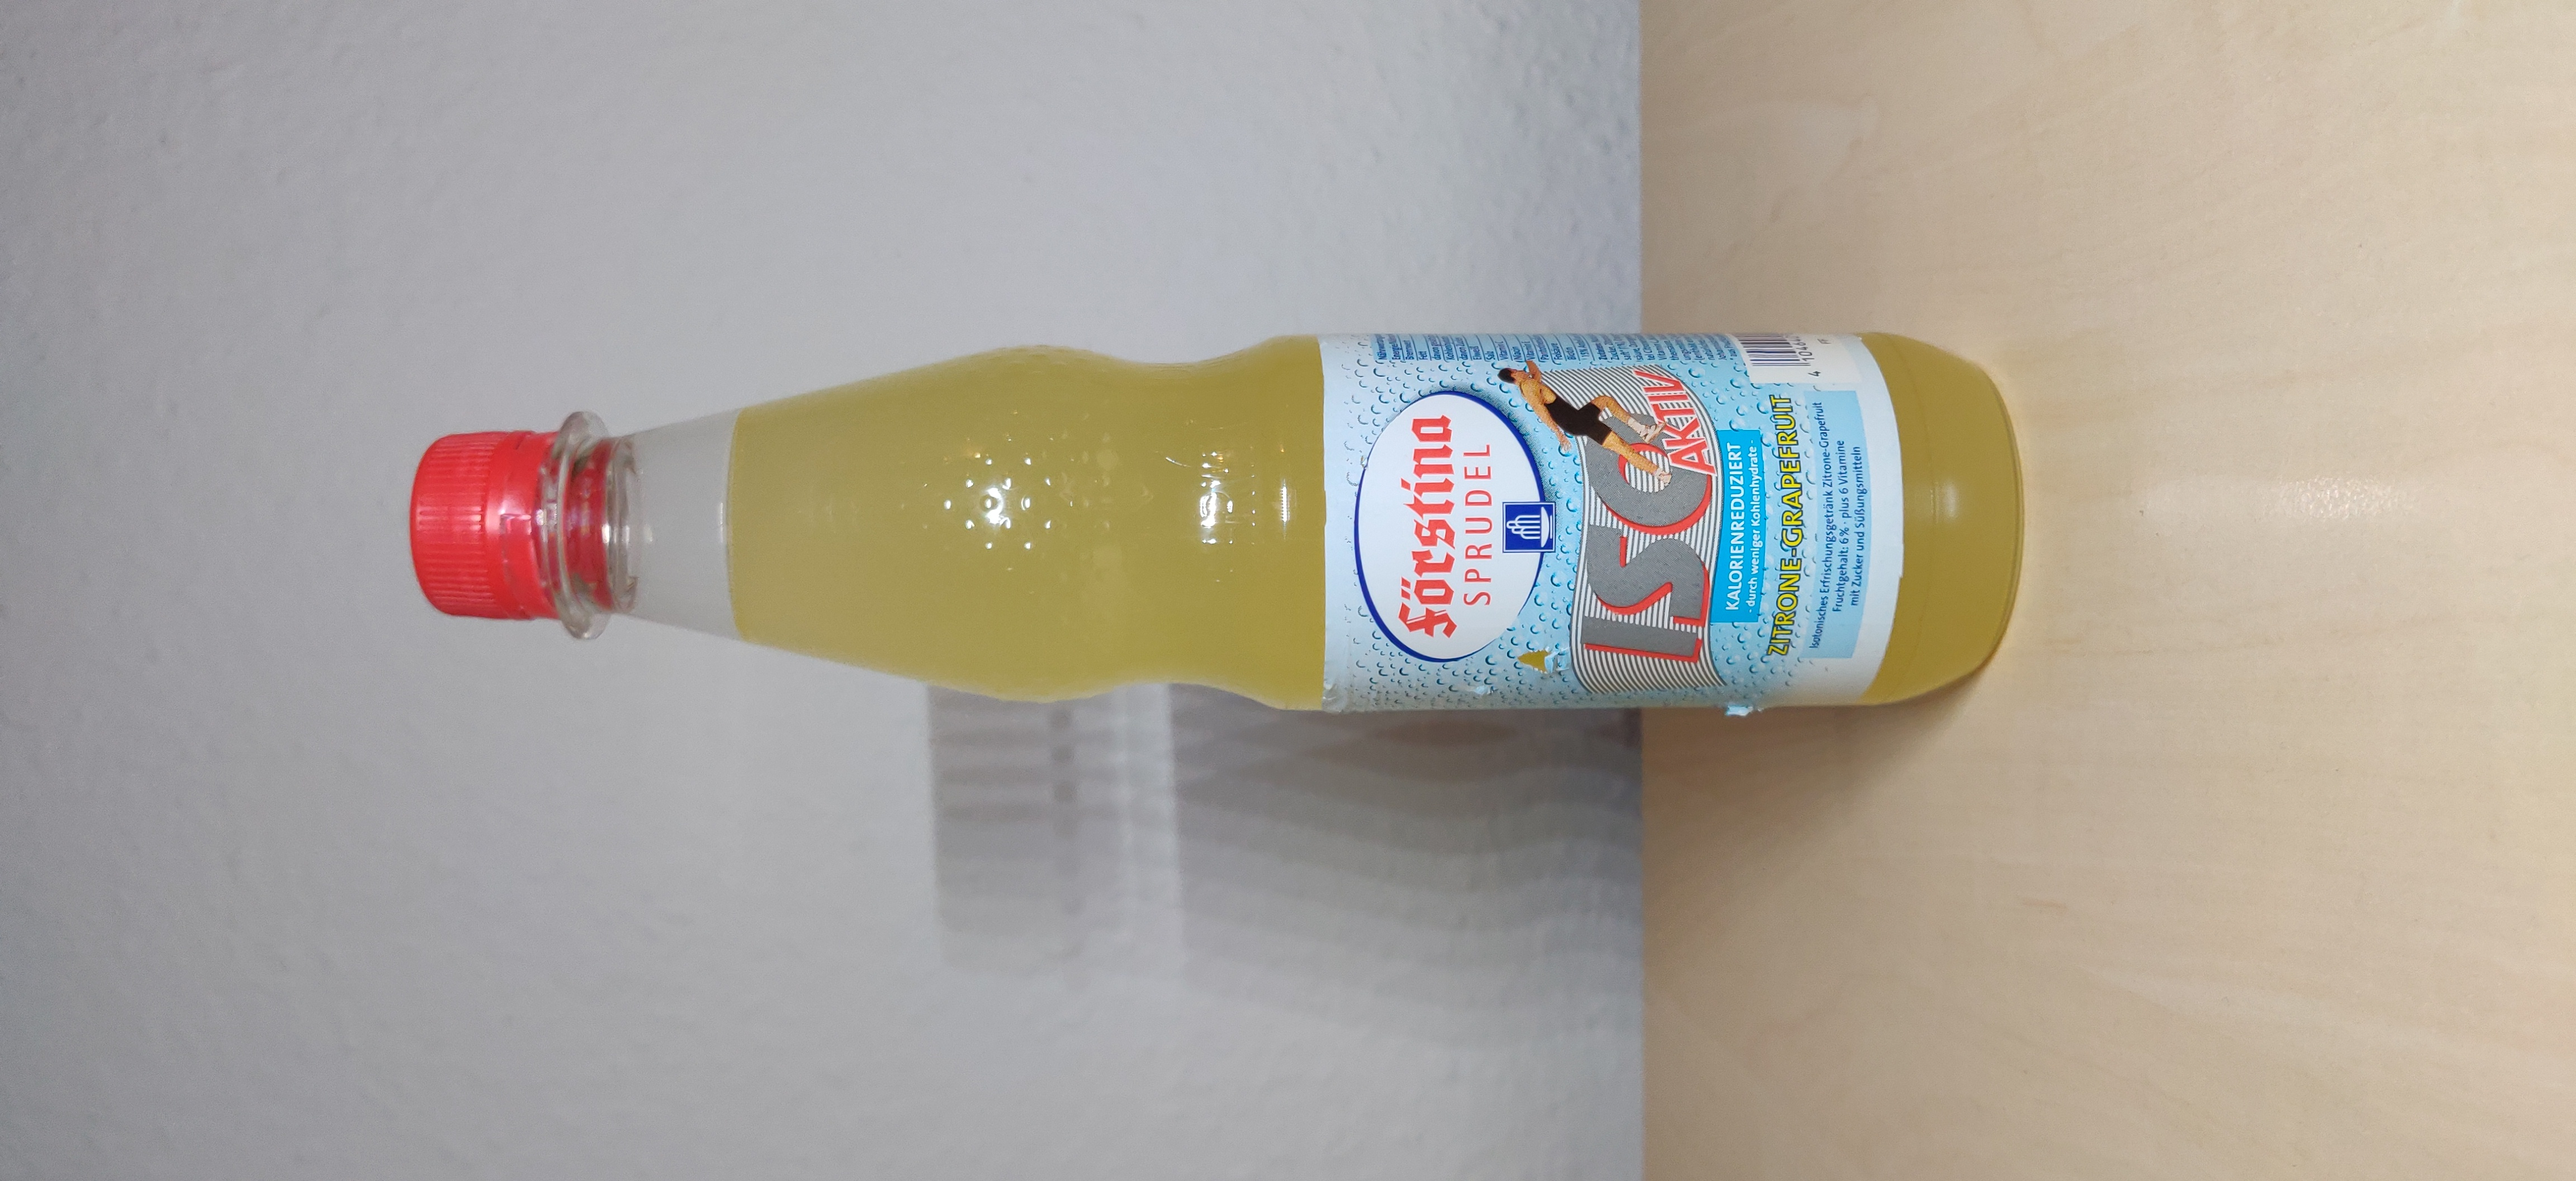
\includegraphics[width=0.30\textwidth]{Bilder/iso.jpg}}\hfill
	\subfigure[ACE]{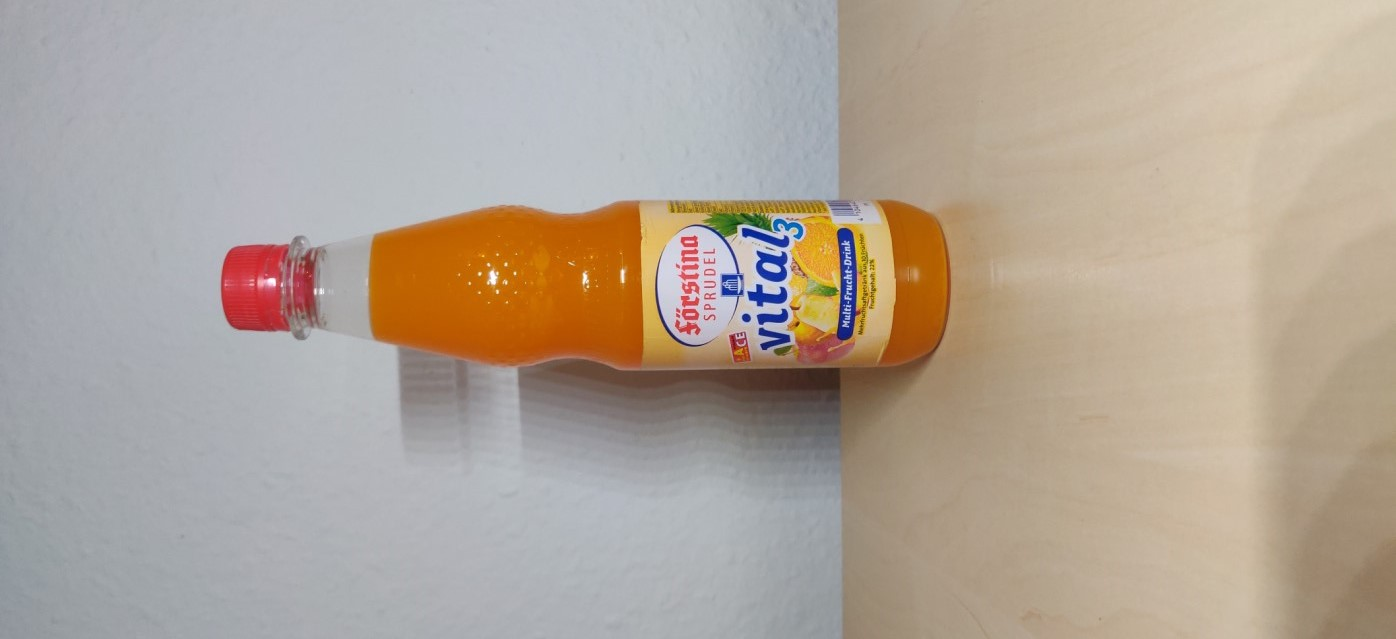
\includegraphics[width=0.30\textwidth]{Bilder/ace.jpg}}\hfill
	\subfigure[Stenger Johannisbeerschorle]{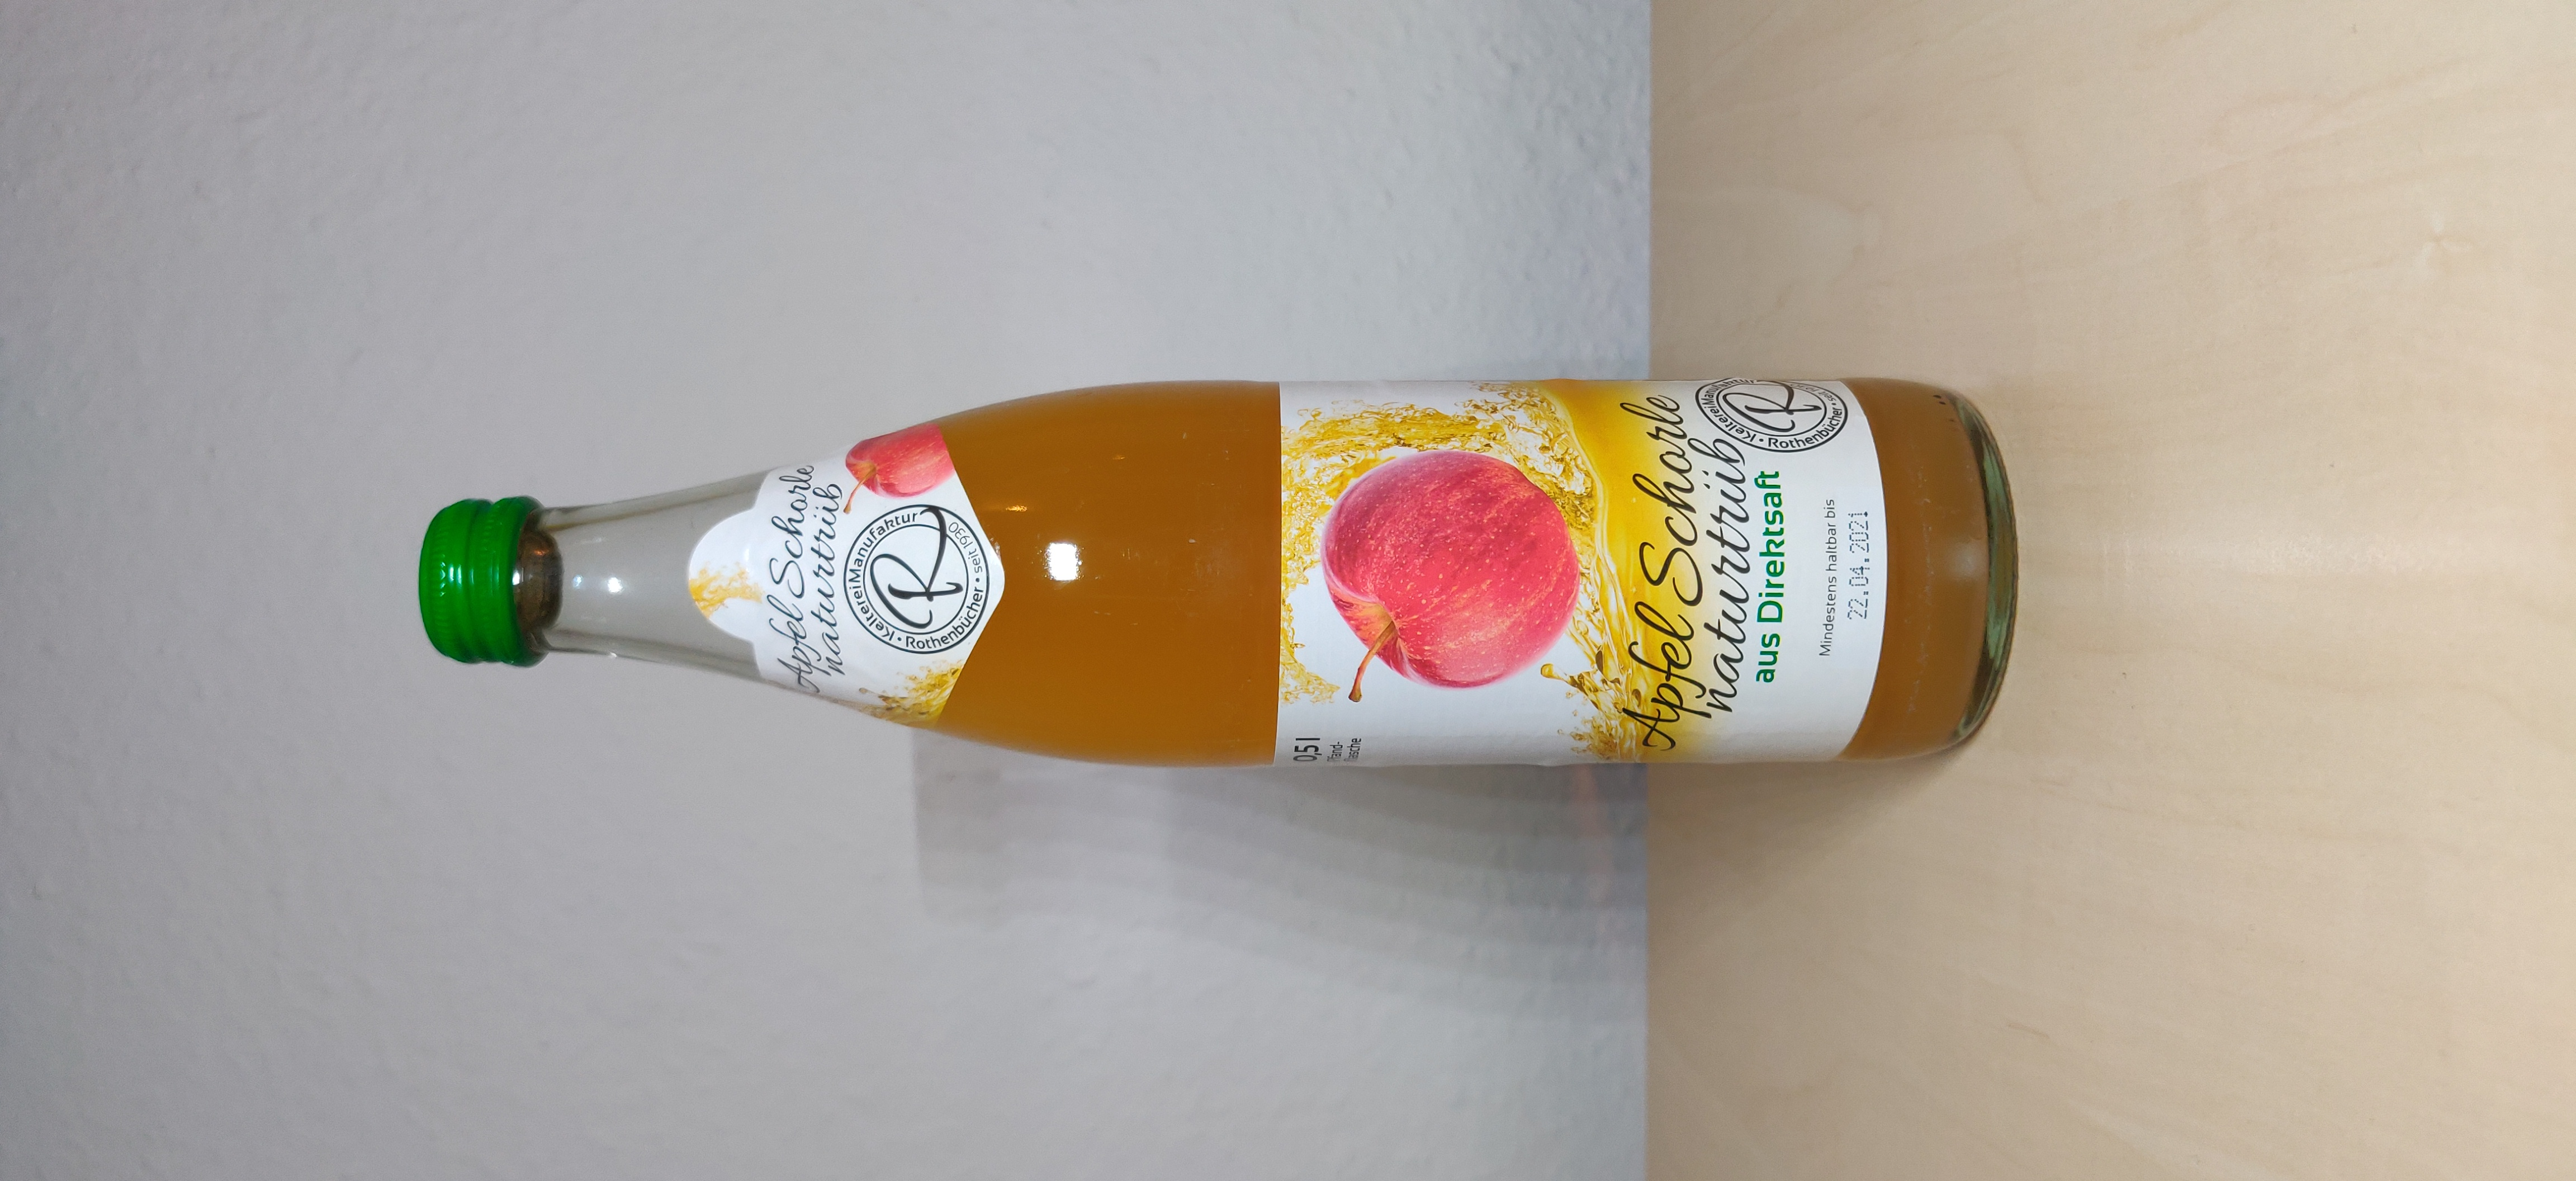
\includegraphics[width=0.30\textwidth]{Bilder/johannisbeerschorle.jpg}}\hfill
	\subfigure[Stenger Apfelsaftschorle]{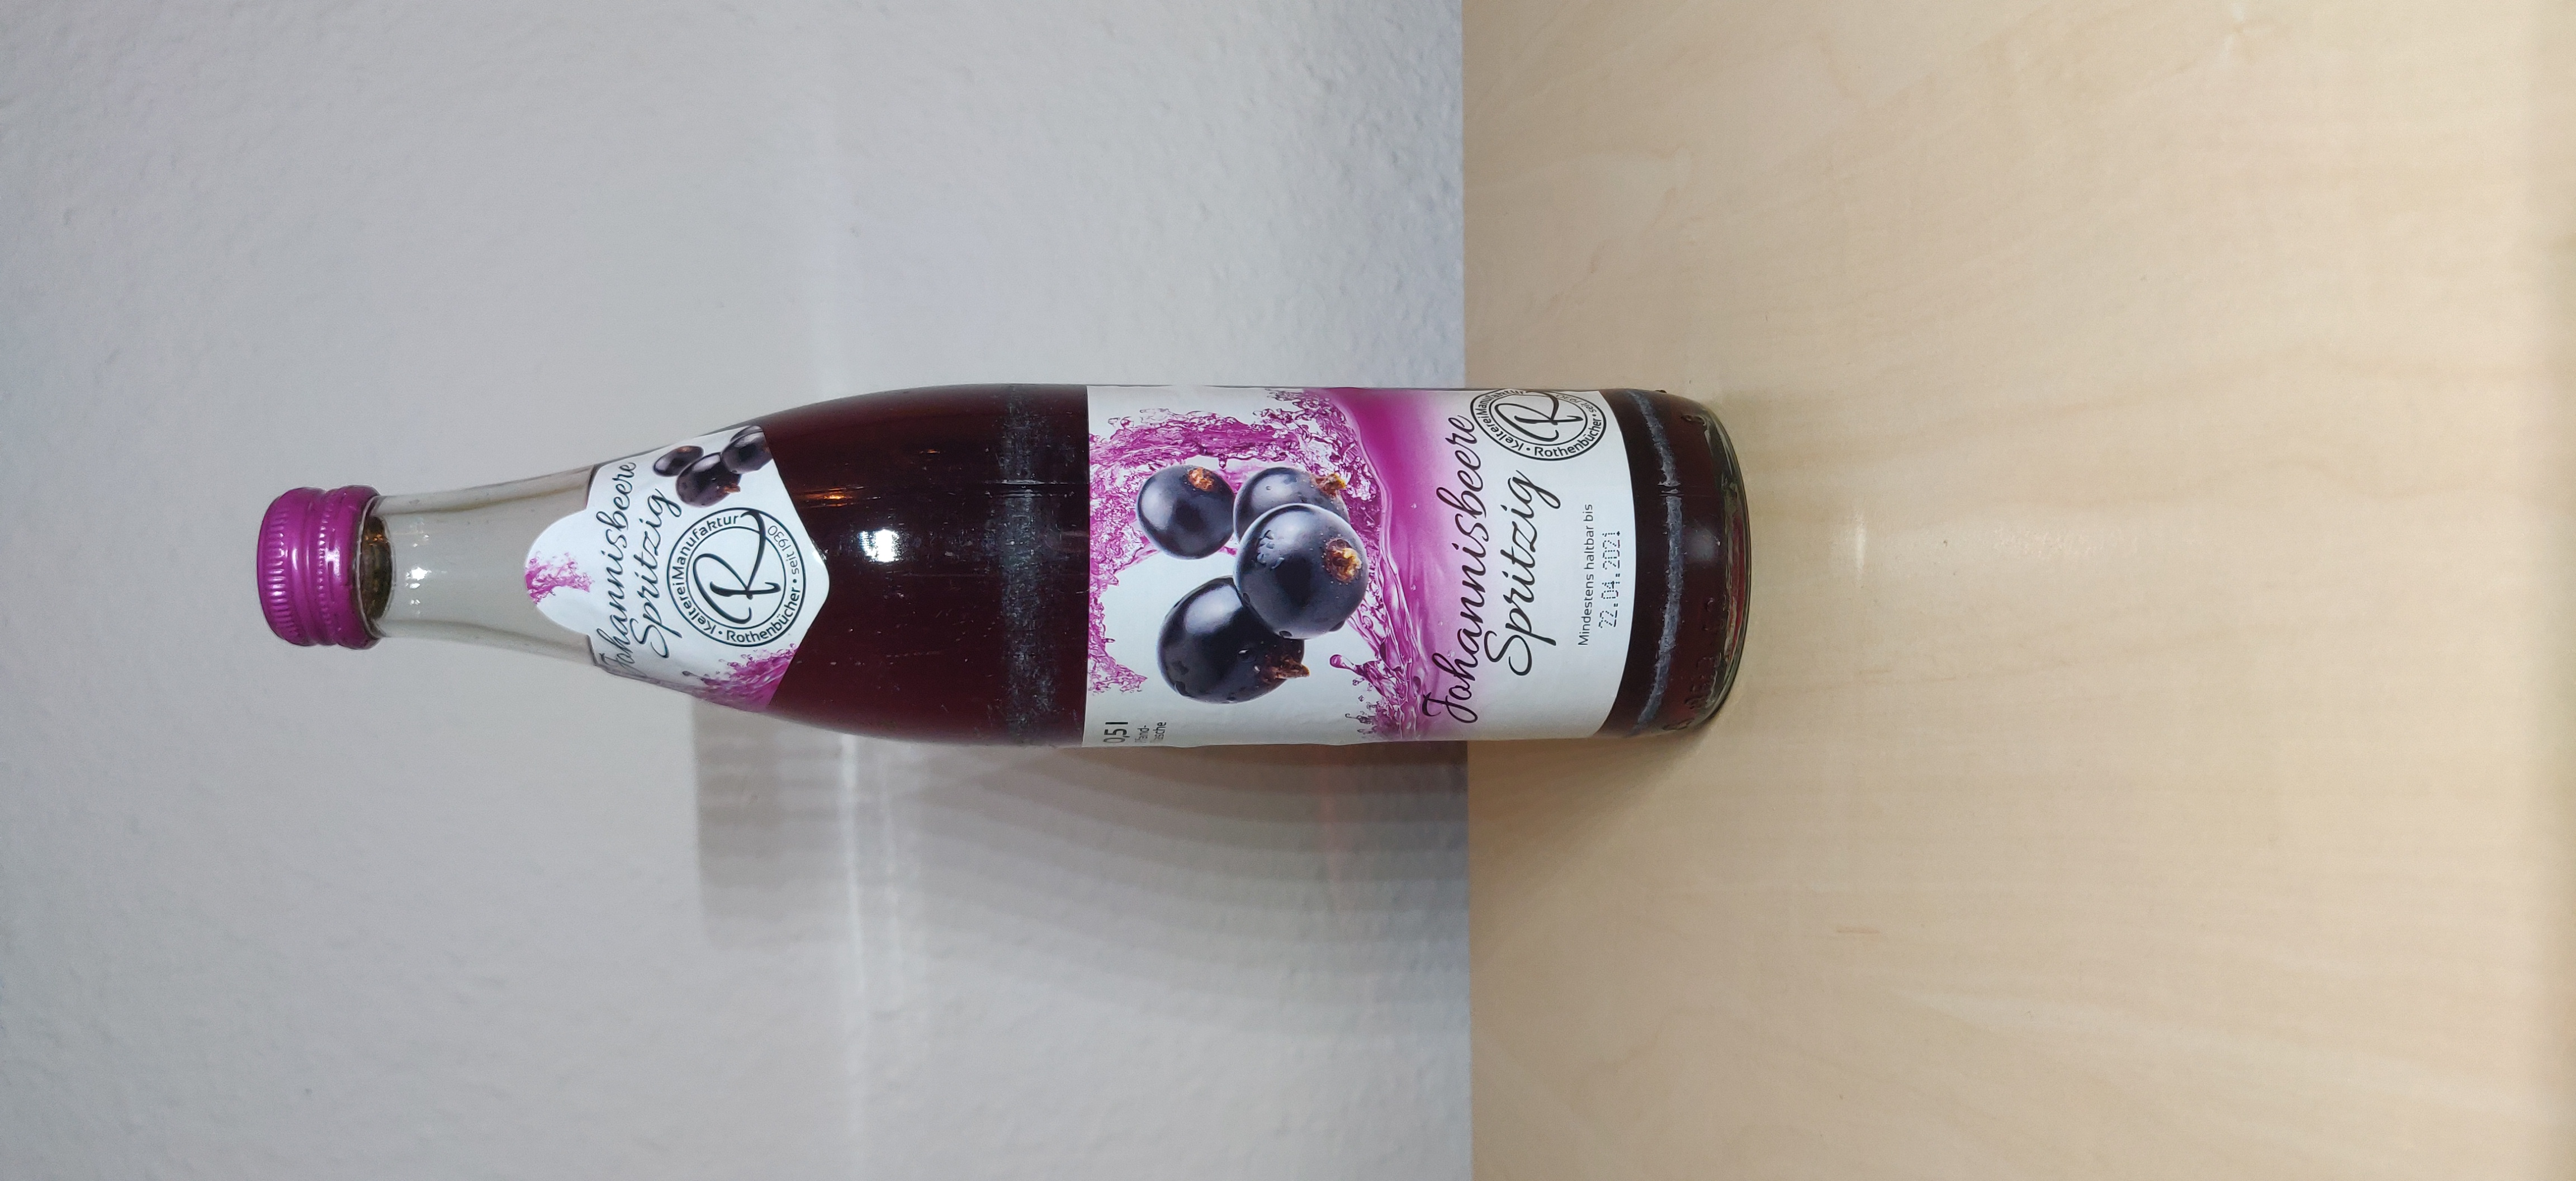
\includegraphics[width=0.30\textwidth]{Bilder/apfelsaftschorle.jpg}}\hfill
	\subfigure[Vitamalz Malzbier]{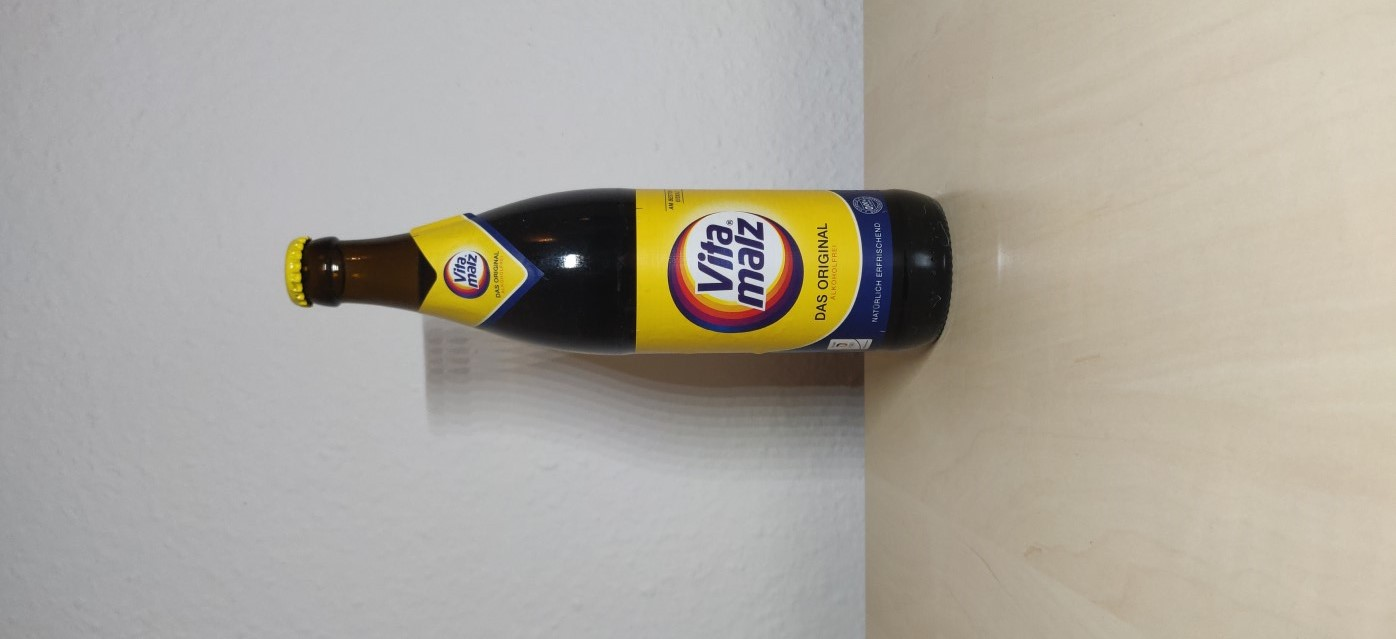
\includegraphics[width=0.30\textwidth]{Bilder/malzbier.jpg}}
	\caption{Die neun Datensatz-Kategorien}
	\label{categories}
\end{figure}

Der Datensatz besteht aus 1000 manuell annotierten Bildern und dient später dazu die ausgewählten Objektdetektoren zu trainieren. Die Bilder besitzen eine Auflösung von 2112x4608 Pixeln mit einer Farbtiefe von 24 Bit. Alle neuen Kategorien sind nahezu gleich häufig im Datensatz vorhanden. Durch das Tool \textit{LabelImg} wurden die Daten sowohl für das \textit{PascalVOC}, als auch das \textit{YOLO} Format annotiert. Im initialen Datensatz sind auf 75\% der Bilder die Objekte der jeweiligen Kategorien einzeln und klar erkennbar abgebildet. Hierdurch wird erhofft, dass Modell zunächst auf die Muster der jeweiligen Objekte zu trainieren. In 12,5\% der Bilder sind die Objekte der jeweiligen Kategorien ebenso einzeln, allerdings mit unterschiedlichen Hintergründen, Beleuchtungsverhältnissen, Blickwinkeln und Entfernungen abgebildet. Je nach Umgebung wurden Bilder dieses Anteils als schwer erkennbar markiert. Um das Warenhaus zu simulieren, sind in den letzten 12,5\% der Bilder die Objekte auf Regalen angeordnet, jeweils hintereinander oder in Getränkekästen (siehe Abbildung \ref{regal}). 

\begin{figure}[ht]
	\begin{center}
		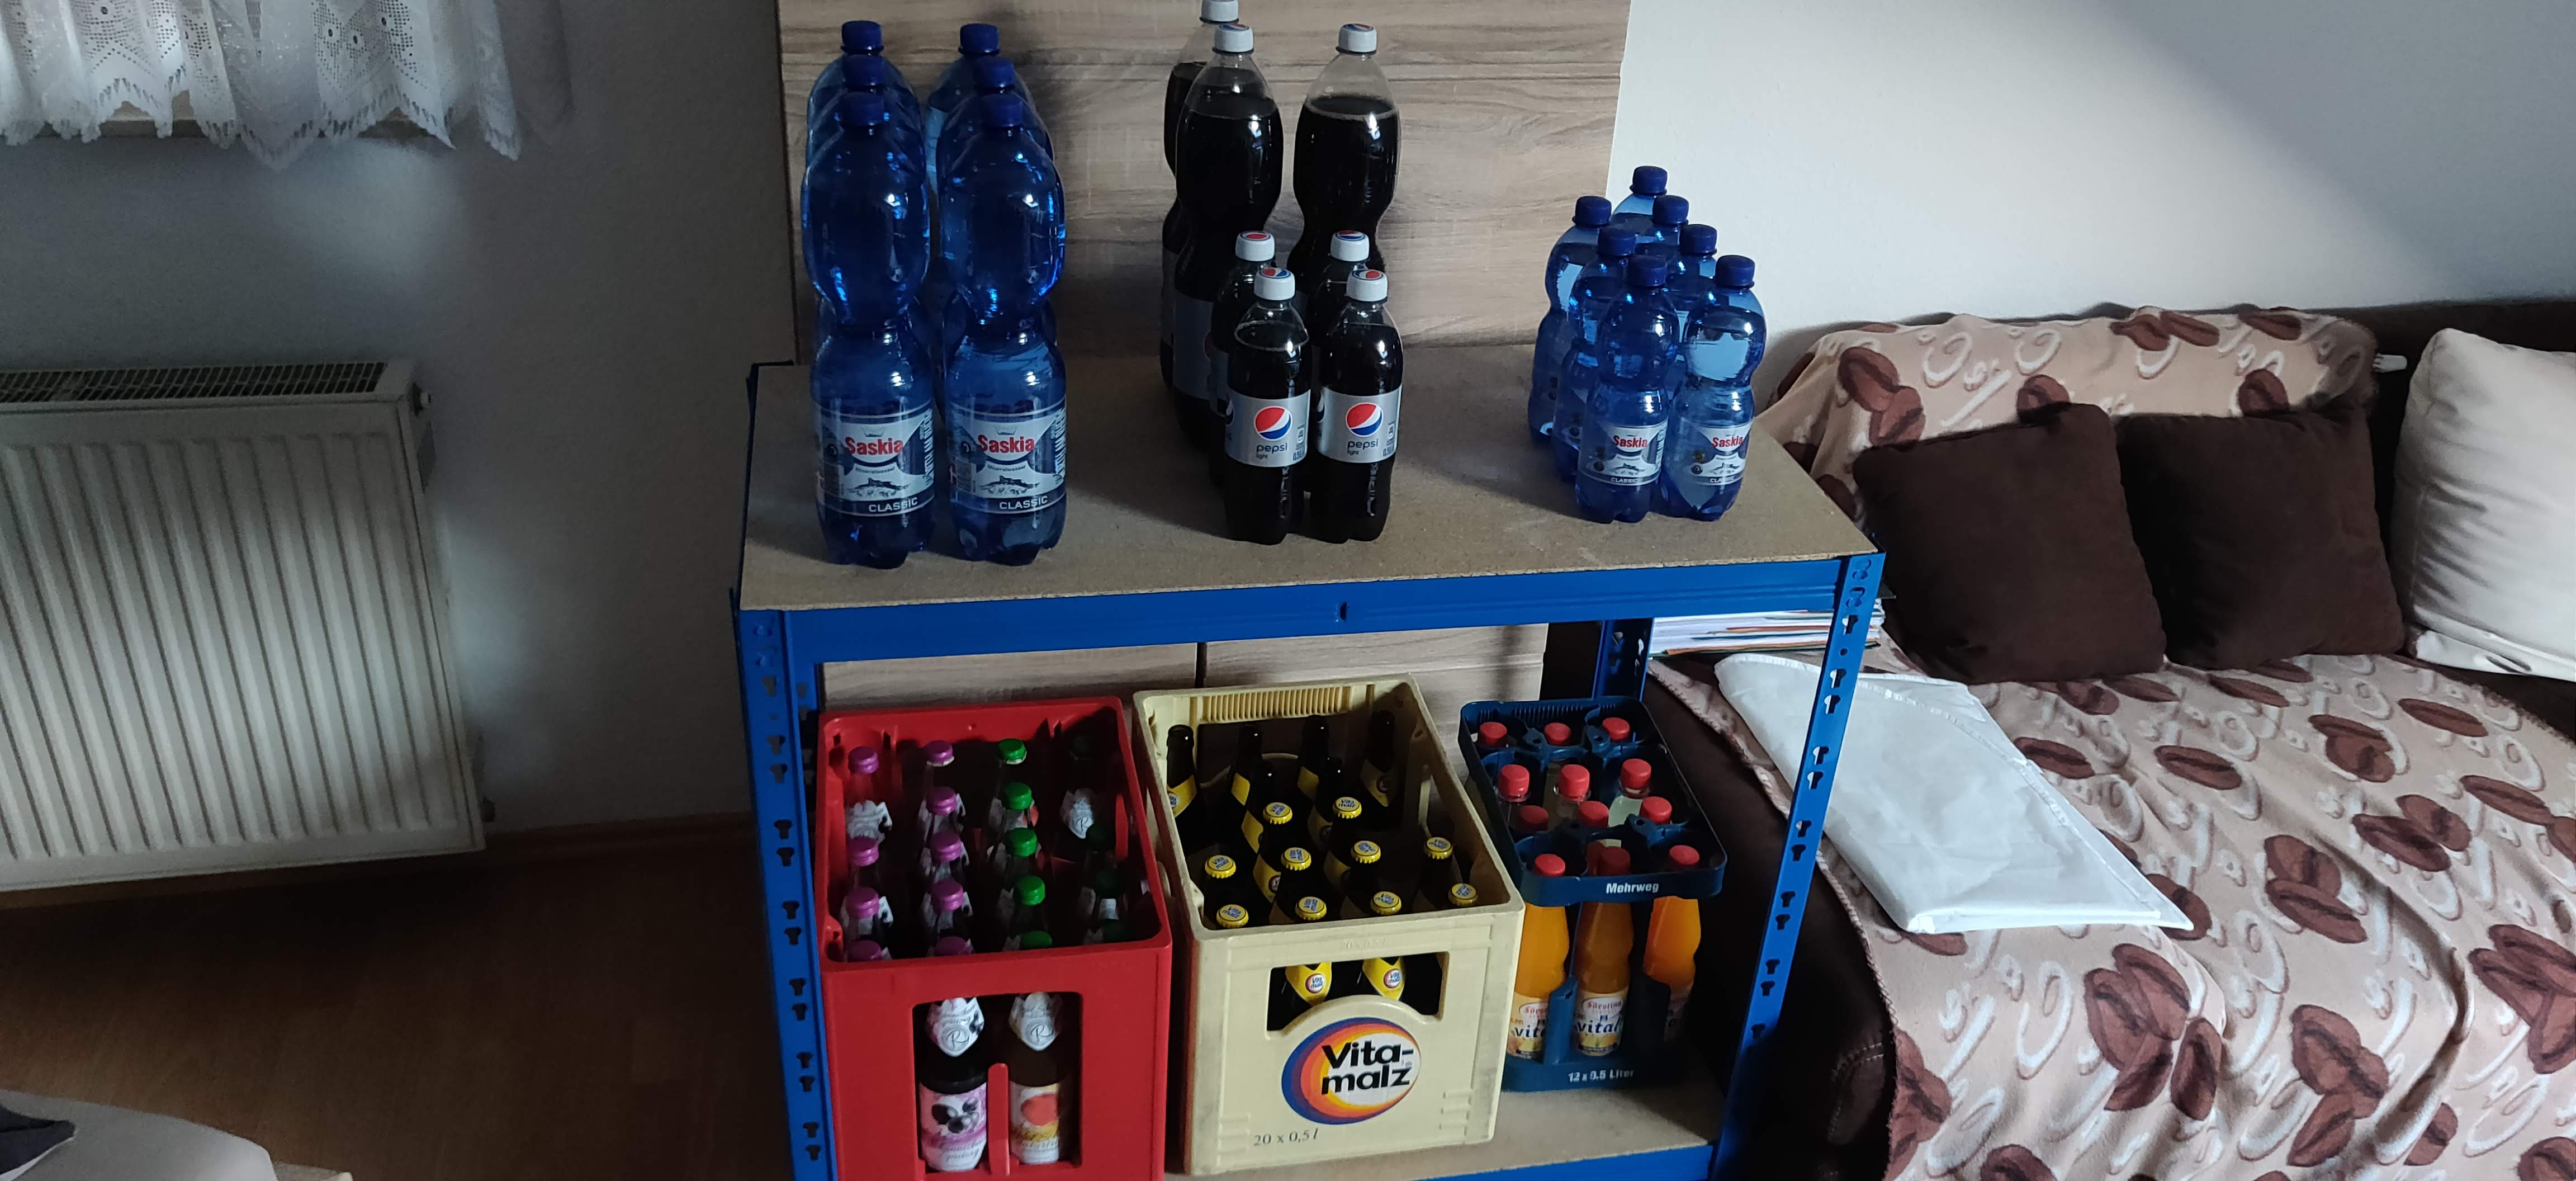
\includegraphics[width=16cm]{Bilder/regal.jpg} 
		\caption[Smart Warehouse Regal]{SmartWarehouse Regal}
		\label{regal}
	\end{center}
\end{figure}